\documentclass[12pt]{article}
\usepackage[top=1in, bottom=1in, left=.75in, right=.75in]{geometry}
\usepackage{amsmath}
\usepackage{fancyhdr}
\usepackage{graphicx}
\usepackage{txfonts}
\usepackage{multicol,coordsys}
\usepackage[scaled=0.86]{helvet}
\renewcommand{\emph}[1]{\textsf{\textbf{#1}}}
\usepackage{anyfontsize}
% \usepackage{times}
% \usepackage[lf]{MinionPro}
\usepackage{tikz,pgfplots,mathrsfs}
%\def\degC{{}^\circ{\rm C}}
\def\ra{\rightarrow}
\usetikzlibrary{calc, backgrounds}
\pgfplotsset{compat = newest}
\newcommand{\blank}[1]{\rule{#1}{0.75pt}}

\pgfplotsset{my style/.append style={axis x line=middle, axis y line=
middle, xlabel={$x$}, ylabel={$y$},axis equal}}

%yticklabels={,,} , xticklabels={,,}

% \setmainfont{Times}
% \def\sansfont{Lucida Grande Bold}
\parindent 0pt
\parskip 4pt
\pagestyle{fancy}
\fancyfoot[C]{\emph{\thepage}}
\fancyhead[L]{\ifnum \value{page} > 1\relax\emph{Math 251: Midterm II}\fi}
\fancyhead[R]{\ifnum \value{page} > 1\relax\emph{Nov 17, 2022}\fi}
\headheight 15pt
\renewcommand{\headrulewidth}{0pt}
\renewcommand{\footrulewidth}{0pt}
\let\ds\displaystyle
\def\continued{{\emph {Continued....}}}
\def\continuing{{\emph {Problem \arabic{probcount} continued....}}\par\vskip 4pt}


\newcounter{probcount}
\newcounter{subprobcount}
\newcommand{\thesubproblem}{\emph{\alph{subprobcount}.}}
\def\problem#1{\setcounter{subprobcount}{0}%
\addtocounter{probcount}{1}{\emph{\arabic{probcount}.\hskip 1em(#1)}}\par}
\def\subproblem#1{\par\hangindent=1em\hangafter=0{%
\addtocounter{subprobcount}{1}\thesubproblem\emph{#1}\hskip 1em}}
\def\probskip{\vskip 10pt}
\def\medprobskip{\vskip 2in}
\def\subprobskip{\vskip 45pt}
\def\bigprobskip{\vskip 4in}

\begin{document}
{\emph{\fontsize{26}{28}\selectfont Math F251\hfill
{\fontsize{32}{36}\selectfont Midterm 2}
\hfill Fall 2022}}
\vskip 2cm
\strut\vtop{\halign{\emph#\hskip 0.5em\hfil&#\hbox to 2in{\hrulefill}\cr
\emph{\fontsize{18}{22}\selectfont Name:}&\cr
\noalign{\vskip 10pt}}}
%%\emph{\fontsize{18}{22}\selectfont Student Id:}&\cr
%%\noalign{\vskip 10pt}
%%\emph{\fontsize{18}{22}\selectfont Calculator Model:}&\cr
%}}
%\hfill
%\vtop{\halign{\emph{\fontsize{18}{22}\selectfont #}\hfil& \emph{\fontsize{18}{22}\selectfont\hskip 0.5ex $\square$ #}\hfil\cr
%Section: & 001 (Jill Faudree)\cr
%\noalign{\vskip 4pt}
%         & 002 (James Gossell)\cr
%\noalign{\vskip 4pt}
%         & 005 (James Gossell)\cr}}

\vfill
{\fontsize{18}{22}\selectfont\emph{Rules:}}

You have 90 minutes to complete the exam.  

Partial credit will be awarded, but you must show your work.

You may have a single handwritten $3 \times 5$ notecard.

Calculators are not allowed. 


Place a box around your  \fbox{FINAL ANSWER} to each question where appropriate.

%If you need extra space, you can use the back sides of the pages.
%Please make it obvious  when you have done so.

Turn off anything that might go beep during the exam.

Good luck!
\vfill
\def\emptybox{\hbox to 2em{\vrule height 16pt depth 8pt width 0pt\hfil}}
\def\tline{\noalign{\hrule}}
\centerline{\vbox{\offinterlineskip
{
\bf\sf\fontsize{18pt}{22pt}\selectfont
\hrule
\halign{
\vrule#&\strut\quad\hfil#\hfil\quad&\vrule#&\quad\hfil#\hfil\quad
&\vrule#&\quad\hfil#\hfil\quad&\vrule#\cr
height 3pt&\omit&&\omit&&\omit&\cr
&Problem&&Possible&&Score&\cr\tline
height 3pt&\omit&&\omit&&\omit&\cr
&1&&10&&\emptybox&\cr\tline
&2&&10&&\emptybox&\cr\tline
&3&&10&&\emptybox&\cr\tline
&4&&10&&\emptybox&\cr\tline
&5&&18&&\emptybox&\cr\tline
&6&&10&&\emptybox&\cr\tline
&7&&10&&\emptybox&\cr\tline
&8&&10&&\emptybox&\cr\tline
&9&&12&&\emptybox&\cr\tline
&Extra Credit&&5&&\emptybox&\cr\tline
&Total&&100&&\emptybox&\cr
}\hrule}}}

\newpage
\begin{enumerate}
%linear approximation
\item (10 points)% \textcolor{red}{Are we OK with this? We were in disagreement and never returned.}
	\begin{enumerate}
	\item Find the linear approximation (also known as the linearization) of the function $f(x)=\sqrt{x}$ when $a=1.$
	\vfill
	\item Use the linear approximation from part (a) to estimate $\sqrt{1.05}$. Your answer must be in the form of a simplified decimal or an exact fraction.
	\vfill
	\end{enumerate}

%lhopitals
\item (10 points) Evaluate the following limits. \textbf{You must show your work and justify your answer to earn full credit.} If you apply L'Hopital's Rule, you should indicate this, by writing $\overset{H}{=}$ or $\overset{L'H}{=}$ or some other clear indication.
	\begin{enumerate}
	\item $\displaystyle{\lim_{x \to \infty} \frac{\sqrt{x^2+4}}{6x+4}}$ 
	\vfill
	\item $\displaystyle{\lim_{x\to 0} \frac{x^2}{4-4\cos(x)}}$
	\vfill
	\end{enumerate}
	

\newpage

%related rate
\item (10 points) The formula for the volume, $V$, of a cone in terms of its radius $r$ and height $h$ is \\$V=\frac{1}{3} \pi r^2 h.$ 
%\begin{enumerate}
%\item Determine the volume of the cone if the radius is 10 cm and the height is 20 cm. Include units with your answer.
%\vspace{1in}
%\item 
If the volume of the cone remains {\bf constant} and the radius of the cone is increasing at a rate of 5 cm/s, determine the rate of change of the height of the cone at the instant the radius is 10 cm and the height is 6 cm. \textbf{Interpret your answer using a compete sentence.} 
%\end{enumerate}
\newpage


%Max/min problem
\item (10 points) Determine the maximum area of a rectangle with base on the $x$-axis inscribed between the parabola $y=12-x^2$ and the $x$-axis (See figure below.) 
Note: Your solution must use Calculus to \emph{justify} that your answer is correct.\\

\def\xx{1}
\begin{tikzpicture}[yscale=.3]
  \draw[->] (-4, 0) -- (4, 0) node[right] {$x$};
  \draw[->] (0, -1) -- (0,14) node[above] {$y$};
  \draw[<->,domain=-4:4, smooth, variable=\x, thick] plot ({\x}, {12-\x*\x});
 \draw[ultra thick] (-\xx,0)--(\xx,0)--(\xx,12-\xx*\xx)--(-\xx,12-\xx*\xx)--(-\xx,0);
 \begin{scope}[on background layer]
 \filldraw[,domain=-sqrt(12):sqrt(12), smooth, variable=\x, thick, opacity=.15] plot ({\x}, {12-\x*\x});
 \end{scope}
\end{tikzpicture}
\hfill

\textbf{answer:} Maximum area is \underline{\hspace{2in}}

%\end{enumerate}

\newpage
%derivative + shape of graph
\item (18 points) Use the information below to answer questions about the function $f(x).$ You must show your work to earn full credit. \\
$$f(x)=\frac{x}{e^x}, \hspace{.2in} f'(x)=\frac{-(x-1)}{e^x},
\hspace{.2in} f''(x)=\frac{x-2}{e^x}.$$

\begin{enumerate}
\item  Determine the intervals on which $f(x)$ is increasing/decreasing.
\vfill
\item Find the $x$-values that correspond to any local maximums or local minimums of $f(x)$. 
\vspace{1in}
\item Find the intervals on which $f(x)$ is concave up and concave down.
\vfill 
\item Find the $x$-values of any inflection points of $f(x).$ If there aren't any, you must explicitly state this and justify your answer.\\

\vspace{1in}

\hfill \textbf{... continued on the next page....}
\newpage
\textbf{... from the previous page....}

Note the function and its derivatives are: 
$$f(x)=\frac{x}{e^x}, \hspace{.2in} f'(x)=\frac{-(x-1)}{e^x},
\hspace{.2in} f''(x)=\frac{x-2}{e^x}.$$


\item Give the equation of any horizontal asymptotes of $f(x)$ or state that none exist. Justify your answer using Calculus. 
\vfill
\item  Give the equation of any vertical asymptotes of $f(x)$ or state that none exist. Justify your answer using  using Calculus. 
\vfill
\end{enumerate}

\newpage

%area under curve
\item (10 points) The function $f(x)=5-2 \ln(x)$ is graphed below. We want to estimate the area under the curve $f(x)$ on the interval $[1,9]$ using $L_4.$ (That is, we want to use 4 approximating rectangles and left-hand end points.) 
\begin{enumerate}
\item Sketch the four approximating rectangles on the graph. 

\begin{tikzpicture}[scale=.8]
\draw[thick, ->] (0,-1) -- (0,6.8);
\draw[thick, ->] (-1,0) -- (10.2,0);
\foreach \j in {1,2,3,4,5,6,7,8,9,10}{
	\draw (\j,-0.15) -- (\j, 0.15);
	\node at (\j,-.5){$\j$};
	}
\foreach \j in {1,2,3,4,5,6}{
	\draw (-0.15,\j) -- (0.15,\j);
	\node at (-0.5,\j){$\j$};
	}
\draw[<->,line width=1.2pt,smooth,samples=100,domain=0.5:10] plot(\x,{5-2*ln((\x))});
\end{tikzpicture}
\vspace{0.5in}
\item Do a calculation to estimate the area under the curve using $L_4$ (that is, use 4 approximating rectangles and left-hand end points) and simplify your answer.  Note: You are obviously not expected to compute things like $\ln(4)$. It is acceptable to have numbers like this in your final answer.\\


\end{enumerate}
\newpage
%antiderivatives
\item (10 points) Evaluate the indefinite integrals below. 
	\begin{enumerate}
	\item $ \displaystyle \int (5\cos(x)+x^{4} + x^{-1}+8) \: dx$
	\vfill
	\item $ \displaystyle \int\frac{1+x^3}{x^2} \: dx $
	\vfill
	\end{enumerate}
	
\item (10 points) Evaluate the definite integrals below using the graph of $f(x)$ and properties of definite integrals. Show your work.

\begin{center}
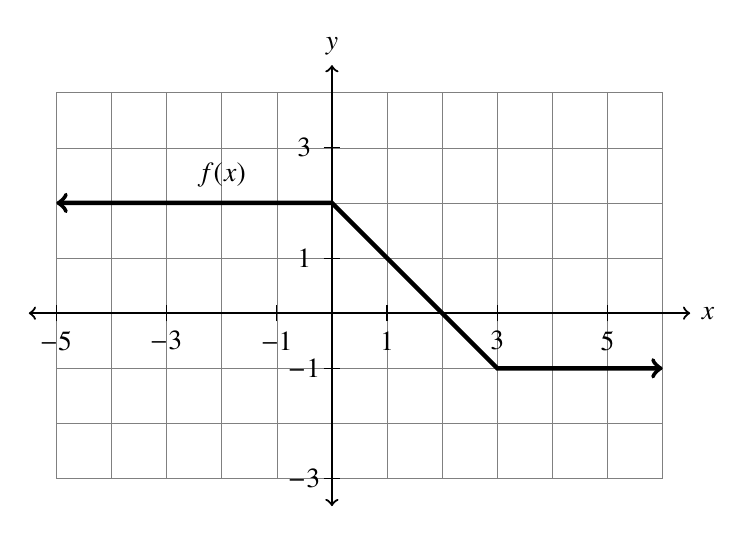
\begin{tikzpicture}[scale=.7]
\draw[help lines] (-5,-3) grid (6, 4);
\draw[<->, thick] (-5.5, 0) -- (6.5, 0) node[right] {$x$};
 \draw[<->, thick] (0, -3.5) -- (0,4.5) node[above] {$y$};
 \draw[<->, ultra thick] (-5,2) -- (0,2) -- (3,-1) -- (6,-1);
% \draw[thick, ->] (0,-1) -- (0,5.8);
%\draw[thick, ->] (-1,0) -- (10.2,0);
\foreach \j in {-5,-3,...,6}{
	\draw (\j,-0.15) -- (\j, 0.15);
	\node at (\j,-.5){$\j$};
	}
\foreach \j in {-3,-1,...,4}{
	\draw (-0.15,\j) -- (0.15,\j);
	\node at (-0.5,\j){$\j$};
	}
\node at (-2,2.5) {$f(x)$};
\end{tikzpicture}
\end{center}

\begin{enumerate}
\item $\displaystyle{\int_{-3}^4 f(x) \: dx}$
\vfill
\item
$\displaystyle{\int_{-3}^4 (2 f(x)+5) \: dx}$
\vfill
\end{enumerate}
\newpage
\item (12 points) Sketch the graph of a function $f(x)$ that satisfies all of the given conditions. Clearly label any important points on the x-axis, draw any asymptotes clearly as dashed lines, and label any asymptotes with their equations.
\begin{enumerate}
\item The domain of $f(x)$ is $(-\infty, \infty).$
\item $f(0)=5$ and $f'(0)$ is undefined
\item $\displaystyle{\lim_{x \to -\infty} f(x)=-1}$
\item $f'(x) >0$ on the interval $(-\infty,0)$; $f'(x) < 0$ on the interval $(0, \infty)$
\item $f''(x) >0$ on the interval $(-\infty, 0)$; $f''(x) <0$ on the interval $(0,\infty)$
\end{enumerate}

\begin{center}
\begin{tikzpicture}[scale=1]
  \draw[->,thick] (-4, 0) -- (4, 0) node[right] {$x$};
  \draw[->,thick] (0, -4) -- (0,4) node[above] {$y$};
%\draw[help lines] (0,0) grid (16, 16);
\end{tikzpicture}
\end{center}



\end{enumerate}

\textbf{Extra Credit:} Suppose $C(t)$ models the position of a car and $B(t)$ models the position of a bike over the same time interval, $[0,2],$ where $C$ and $B$ are measured in miles and $t$ in hours.\\
(3 pts) Translate the following sentence into the language of Calculus: "The car goes faster than the bike but the bike accelerates faster than the car." (i.e. rewrite the sentence using derivatives in some form.)\\
(2pts) Construct a pair of functions $C(t)$ and $B(t)$ satisfying the properties described in the sentence on the interval $[0,2].$ (Note, your functions do not have to be realistic...)

\vspace{4in}
\end{document}
